\documentclass[11pt,letterpaper]{article}

\usepackage[margin=1in]{geometry}
\usepackage{amsmath,amssymb}
\usepackage{graphicx}
\usepackage{booktabs}
\usepackage{array}
\usepackage{xcolor}
\usepackage{listings}
\usepackage{tikz}
\usetikzlibrary{positioning,arrows.meta,fit,backgrounds,calc,decorations.pathreplacing}
\usepackage{hyperref}
\usepackage{enumitem}
\usepackage{fancyvrb}
\usepackage{caption}
\usepackage{subcaption}
\usepackage{longtable}
\usepackage{multirow}

% Colors
\definecolor{cpuBlue}{HTML}{2563EB}
\definecolor{wseColor}{HTML}{0891B2}
\definecolor{confirmGreen}{HTML}{059669}
\definecolor{conflictRed}{HTML}{DC2626}
\definecolor{warnOrange}{HTML}{D97706}
\definecolor{codeBg}{HTML}{F3F4F6}
\definecolor{codeFrame}{HTML}{D1D5DB}
\definecolor{pe0color}{HTML}{DBEAFE}
\definecolor{pe1color}{HTML}{D1FAE5}
\definecolor{pe2color}{HTML}{FEF3C7}
\definecolor{pe3color}{HTML}{FEE2E2}

% Listings style
\lstset{
  basicstyle=\ttfamily\small,
  backgroundcolor=\color{codeBg},
  frame=single,
  rulecolor=\color{codeFrame},
  breaklines=true,
  numbers=left,
  numberstyle=\tiny\color{gray},
  xleftmargin=18pt,
  xrightmargin=4pt,
  aboveskip=8pt,
  belowskip=8pt,
  columns=fullflexible,
  keepspaces=true,
  escapeinside={(*@}{@*)},
}

\lstdefinelanguage{CSL}{
  morekeywords={fn,var,const,param,task,comptime,while,if,else,return,inline,void,bool,true,false,break,continue,for},
  morekeywords=[2]{i16,i32,u16,u32,f32,color,input_queue,output_queue,local_task_id,data_task_id},
  morekeywords=[3]{@activate,@block,@unblock,@bind_local_task,@bind_data_task,@export_symbol,@export_name,@get_color,@import_module,@set_tile_code,@set_color_config,@mov32,@get_dsd,@bitcast,@as,@zeros,@is_arch},
  sensitive=true,
  morecomment=[l]{//},
  morestring=[b]",
  keywordstyle=\color{cpuBlue}\bfseries,
  keywordstyle=[2]\color{wseColor},
  keywordstyle=[3]\color{warnOrange},
  commentstyle=\color{gray}\itshape,
  stringstyle=\color{confirmGreen},
}

\lstdefinelanguage{PyHost}{
  morekeywords={def,class,import,from,for,while,if,else,return,with,as,in,range,True,False,None,print,open,int,str,float,list,dict,np},
  morekeywords=[2]{SdkRuntime,MemcpyDataType,MemcpyOrder,memcpy_h2d,memcpy_d2h,calculate_cycles,get_id,load,run,launch,stop},
  sensitive=true,
  morecomment=[l]{\#},
  morestring=[b]",
  morestring=[b]',
  keywordstyle=\color{cpuBlue}\bfseries,
  keywordstyle=[2]\color{wseColor},
  commentstyle=\color{gray}\itshape,
  stringstyle=\color{confirmGreen},
}

\title{\textbf{Picasso: Graph Coloring on the Cerebras WSE}\\[4pt]\large An End-to-End Walkthrough}
\author{Siddharth Banakar}
\date{}

\begin{document}
\maketitle

\tableofcontents
\newpage

%======================================================================
\section{System Architecture Overview}
\label{sec:overview}
%======================================================================

The implementation has three layers, each with a clear job:

\begin{center}
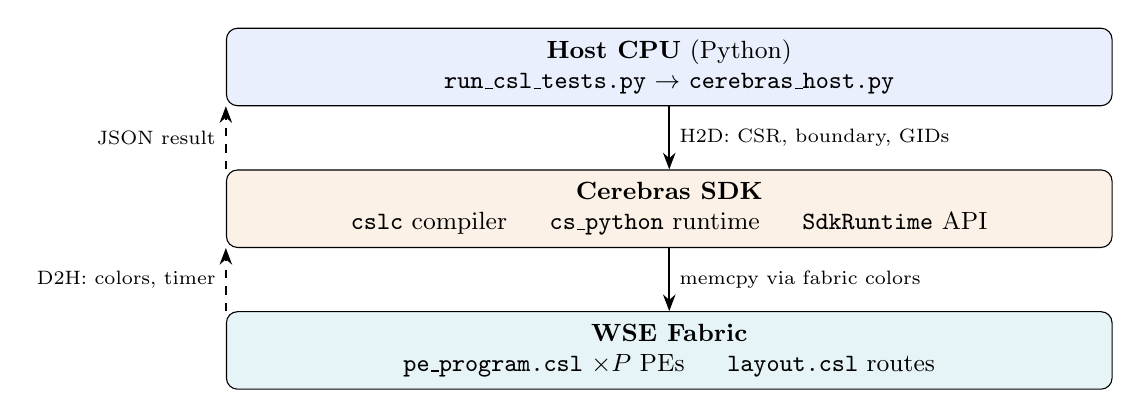
\begin{tikzpicture}[
    box/.style={draw, rounded corners=4pt, minimum width=100pt, minimum height=28pt, font=\small, align=center},
    arrow/.style={-{Stealth[length=6pt]}, thick},
    xscale=1.1
  ]
  % Host layer
  \node[box, fill=cpuBlue!10, minimum width=320pt] (host) at (0,4)
    {\textbf{Host CPU} (Python)\\
     \texttt{run\_csl\_tests.py} $\to$ \texttt{cerebras\_host.py}};

  % SDK layer
  \node[box, fill=warnOrange!10, minimum width=320pt] (sdk) at (0,2.2)
    {\textbf{Cerebras SDK}\\
     \texttt{cslc} compiler $\quad$ \texttt{cs\_python} runtime $\quad$ \texttt{SdkRuntime} API};

  % Device layer
  \node[box, fill=wseColor!10, minimum width=320pt] (device) at (0,0.4)
    {\textbf{WSE Fabric}\\
     \texttt{pe\_program.csl} $\times P$ PEs $\quad$ \texttt{layout.csl} routes};

  \draw[arrow] (host.south) -- node[right,font=\scriptsize] {H2D: CSR, boundary, GIDs} (sdk.north);
  \draw[arrow] (sdk.south) -- node[right,font=\scriptsize] {memcpy via fabric colors} (device.north);
  \draw[arrow, dashed] (device.north west) -- node[left,font=\scriptsize] {D2H: colors, timer} (sdk.south west);
  \draw[arrow, dashed] (sdk.north west) -- node[left,font=\scriptsize] {JSON result} (host.south west);
\end{tikzpicture}
\end{center}

\subsection{File Map}

\begin{center}
\renewcommand{\arraystretch}{1.2}
\begin{tabular}{lll}
\toprule
\textbf{File} & \textbf{Language} & \textbf{Role} \\
\midrule
\texttt{picasso/run\_csl\_tests.py} & Python & Test orchestrator: loads Paulis, builds CSR, partitions, compiles, runs \\
\texttt{picasso/cerebras\_host.py}  & Python & Runs inside \texttt{cs\_python} container; uploads data, launches kernel \\
\texttt{csl/layout.csl}            & CSL    & Fabric layout: PE grid, color routes, sync barrier wiring \\
\texttt{csl/pe\_program.csl}       & CSL    & PE kernel: speculate, send, recv, barrier, detect/resolve \\
\texttt{tests/inputs/*.json}       & JSON   & Pauli string test inputs \\
\bottomrule
\end{tabular}
\end{center}

\subsection{The Running Example}

Throughout this document we follow a concrete example: the 12-vertex graph from \texttt{test6\_12nodes.json}. The raw data is a set of 8-qubit Pauli strings from a molecular Hamiltonian fragment:

\begin{center}
\begin{tabular}{clcl}
\toprule
\textbf{ID} & \textbf{Pauli String} & \textbf{ID} & \textbf{Pauli String} \\
\midrule
$v_0$  & \texttt{IIXIIIII} & $v_6$  & \texttt{XIIIIIII} \\
$v_1$  & \texttt{IIYIIIII} & $v_7$  & \texttt{XXIIIIII} \\
$v_2$  & \texttt{IIZIIIII} & $v_8$  & \texttt{YIIIIIII} \\
$v_3$  & \texttt{IXIIIIII} & $v_9$  & \texttt{YYIIIIII} \\
$v_4$  & \texttt{IYIIIIII} & $v_{10}$ & \texttt{ZIIIIIII} \\
$v_5$  & \texttt{IZIIIIII} & $v_{11}$ & \texttt{ZZIIIIII} \\
\bottomrule
\end{tabular}
\end{center}

The resulting graph has 12 vertices, 45 edges, and an average degree of~7.5. Most vertices are neighbors of most others, so this is far from a toy problem.

%======================================================================
\section{Stage 1: Pauli Commutativity \texorpdfstring{$\to$}{to} Conflict Graph}
\label{sec:commutativity}
%======================================================================

\subsection{The Commutativity Rule}

Two Pauli strings \emph{commute} when the number of qubit positions where both are non-identity and different is \textbf{even}; otherwise they \emph{anti-commute}. Commuting pairs become edges in our conflict graph---they can share a color group, so the coloring algorithm needs to keep track of them.

\begin{lstlisting}[language=Python, caption={Commutativity check (from \texttt{run\_csl\_tests.py})}, label=lst:commute]
def is_an_edge(s1, s2):
    """True if two Pauli strings anti-commute."""
    count = 0
    for c1, c2 in zip(s1, s2):
        if c1 != 'I' and c2 != 'I' and c1 != c2:
            count += 1
    return count % 2 == 1
\end{lstlisting}

\subsection{Worked Example: \texorpdfstring{$v_0$}{v0} = IIXIIIII vs.\ \texorpdfstring{$v_3$}{v3} = IXIIIIII}

\begin{center}
\begin{tabular}{ccccccccl}
\toprule
Q7 & Q6 & Q5 & Q4 & Q3 & Q2 & Q1 & Q0 & \\
\midrule
I & I & X & I & I & I & I & I & $v_0$ \\
I & X & I & I & I & I & I & I & $v_3$ \\
\midrule
\checkmark & -- & -- & \checkmark & \checkmark & \checkmark & \checkmark & \checkmark & \\
\bottomrule
\end{tabular}
\end{center}

Position Q6: $v_0{=}\text{I}$ (identity, skip). Position Q5: $v_0{=}\text{X}, v_3{=}\text{I}$ (one identity, skip). No positions have both non-identity \emph{and} different. Count $= 0$ (even) $\Rightarrow$ they \textbf{commute} $\Rightarrow$ edge $(v_0, v_3)$ exists.

\subsection{Result: Dense Conflict Graph}

The $\binom{12}{2} = 66$ pairs yield \textbf{45 commuting pairs} (edges) and 21 anti-commuting pairs (no edge). The resulting graph is dense: average degree $= 2 \times 45 / 12 = 7.5$.

\begin{lstlisting}[language=Python, caption={Graph construction (from \texttt{run\_csl\_tests.py})}, label=lst:buildgraph]
def build_conflict_graph(paulis):
    n = len(paulis)
    edges = []
    num_commuting = 0
    for i in range(n - 1):
        for j in range(i + 1, n):
            if not is_an_edge(paulis[i], paulis[j]):
                edges.append((i, j))
                num_commuting += 1
    return n, edges, num_commuting
\end{lstlisting}

%======================================================================
\section{Stage 2: CSR Construction}
\label{sec:csr}
%======================================================================

\subsection{From Edge List to CSR}

The 45 undirected edges become 90 directed arcs (one in each direction) and get packed into two flat arrays---\texttt{offsets[13]} and \texttt{adj[90]}:

\begin{lstlisting}[language=Python, caption={CSR builder (from \texttt{run\_csl\_tests.py})}, label=lst:csr]
def build_csr(num_verts, edges):
    from collections import defaultdict
    adj_list = defaultdict(list)
    for u, v in edges:
        adj_list[u].append(v)
        adj_list[v].append(u)        # symmetric
    offsets = [0]
    adj = []
    for v in range(num_verts):
        neighbors = sorted(adj_list[v])
        adj.extend(neighbors)
        offsets.append(len(adj))
    return np.array(offsets, dtype=np.int32), np.array(adj, dtype=np.int32)
\end{lstlisting}

\subsection{Concrete Arrays for Our 12-Node Graph}

\begin{lstlisting}[numbers=none, caption={CSR arrays for test6\_12nodes}]
offsets = [0, 9, 18, 27, 34, 41, 48, 55, 62, 69, 76, 83, 90]

adj = [3,4,5,6,7,8,9,10,11,    (*@\textcolor{gray}{// $v_0$: 9 neighbors}@*)
       3,4,5,6,7,8,9,10,11,    (*@\textcolor{gray}{// $v_1$: 9 neighbors}@*)
       3,4,5,6,7,8,9,10,11,    (*@\textcolor{gray}{// $v_2$: 9 neighbors}@*)
       0,1,2,6,7,8,10,         (*@\textcolor{gray}{// $v_3$: 7 neighbors}@*)
       0,1,2,6,8,9,10,         (*@\textcolor{gray}{// $v_4$: 7 neighbors}@*)
       0,1,2,6,8,10,11,        (*@\textcolor{gray}{// $v_5$: 7 neighbors}@*)
       0,1,2,3,4,5,7,          (*@\textcolor{gray}{// $v_6$: 7 neighbors}@*)
       0,1,2,3,6,9,11,         (*@\textcolor{gray}{// $v_7$: 7 neighbors}@*)
       0,1,2,3,4,5,9,          (*@\textcolor{gray}{// $v_8$: 7 neighbors}@*)
       0,1,2,4,7,8,11,         (*@\textcolor{gray}{// $v_9$: 7 neighbors}@*)
       0,1,2,3,4,5,11,         (*@\textcolor{gray}{// $v_{10}$: 7 neighbors}@*)
       0,1,2,5,7,9,10]         (*@\textcolor{gray}{// $v_{11}$: 7 neighbors}@*)
\end{lstlisting}

\paragraph{Lookup example: neighbors of $v_6$.}
\[
  \texttt{offsets}[6] = 48, \quad \texttt{offsets}[7] = 55 \quad\Longrightarrow\quad \texttt{adj}[48..55) = [0,1,2,3,4,5,7]
\]
Seven neighbors, found with two integer lookups and one contiguous scan.

\subsection{Memory Cost}

\begin{center}
\begin{tabular}{lr}
\toprule
\textbf{Array} & \textbf{Size (bytes)} \\
\midrule
\texttt{offsets[13]} & $13 \times 4 = 52$ \\
\texttt{adj[90]}    & $90 \times 4 = 360$ \\
\midrule
\textbf{Total CSR} & 412 bytes \\
\bottomrule
\end{tabular}
\end{center}

For comparison, a $12 \times 12$ adjacency matrix would need 144 bytes (booleans only), but CSR wins hands-down for larger sparse graphs and avoids pointer overhead entirely.

%======================================================================
\section{Stage 3: Graph Partitioning Across PEs}
\label{sec:partition}
%======================================================================

This is the critical bridge between the host CPU and the Cerebras fabric. The partitioner splits the graph so that each PE gets:
\begin{itemize}[nosep]
  \item A \textbf{local CSR} with only its own vertices and all their edges
  \item A \textbf{boundary table} listing every edge that crosses to another PE, plus routing info
\end{itemize}

\subsection{Vertex Assignment: Hash-Based Partitioning}

Vertices go to PEs using a simple \textbf{hash}: $\texttt{pe} = \texttt{gid} \mathbin{\&} (\texttt{total\_pes} - 1)$. The PE count must be a power of~2. This distributes vertices evenly and avoids the load imbalance you get with contiguous chunking when high-degree hubs cluster in one partition.

With 2~PEs (1D layout), vertex $v_i$ maps to PE\,$= i \mathbin{\&} 1$---even-numbered vertices go to PE\,0, odd to PE\,1:

\begin{center}
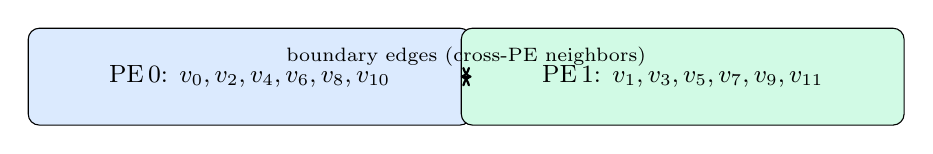
\begin{tikzpicture}[
    pe/.style={draw, rounded corners=4pt, minimum width=160pt, minimum height=35pt, font=\small},
  ]
  \node[pe, fill=pe0color] (pe0) at (0,0)
    {PE\,0: $v_0, v_2, v_4, v_6, v_8, v_{10}$};
  \node[pe, fill=pe1color] (pe1) at (5.5,0)
    {PE\,1: $v_1, v_3, v_5, v_7, v_9, v_{11}$};
  \draw[<->,thick,dashed] (pe0.east)--(pe1.west)
    node[midway,above,font=\scriptsize] {boundary edges (cross-PE neighbors)};
\end{tikzpicture}
\end{center}

\begin{lstlisting}[language=Python, caption={Hash-based vertex-to-PE assignment (from \texttt{run\_csl\_tests.py})}, label=lst:assign]
total_pes = num_cols * num_rows
assert total_pes & (total_pes - 1) == 0  # must be power of 2
pe_mask = total_pes - 1

def gid_to_pe(gid):
    return gid & pe_mask
# 2 PEs: v0,v2,v4,v6,v8,v10 -> PE 0;  v1,v3,v5,v7,v9,v11 -> PE 1
\end{lstlisting}

\subsection{Local CSR Construction}

Each PE gets a \emph{local} CSR that contains \textbf{all} edges of its vertices---including edges to remote vertices: 

\begin{lstlisting}[numbers=none, caption={PE\,0's local CSR (6 vertices, 46 adjacency entries)}]
PE 0 local_offsets = [0, 9, 18, 25, 32, 39, 46]
PE 0 local_adj = [3,4,5,6,7,8,9,10,11,  // v0  (global id 0): 9 neighbors
                  3,4,5,6,7,8,9,10,11,  // v2  (global id 2): 9 neighbors
                  0,1,2,6,8,9,10,        // v4  (global id 4): 7 neighbors
                  0,1,2,3,4,5,7,         // v6  (global id 6): 7 neighbors
                  0,1,2,3,4,5,9,         // v8  (global id 8): 7 neighbors
                  0,1,2,3,4,5,11]        // v10 (global id 10): 7 neighbors
\end{lstlisting}

Notice that the adjacency array stores \emph{global} vertex IDs (not PE-local indices). This allows the PE kernel to match incoming wavelets by global ID. Each PE also receives a \texttt{global\_vertex\_ids[]} array mapping local index $\to$ global ID, and a \texttt{pe\_mask} value for computing $\texttt{dest\_pe} = \texttt{gid} \mathbin{\&} \texttt{pe\_mask}$ at runtime.

\subsection{Boundary Table Construction}

For every edge where the neighbor lives on a different PE, the partitioner records three fields:

\begin{center}
\renewcommand{\arraystretch}{1.2}
\begin{tabular}{ll}
\toprule
\textbf{Field} & \textbf{Meaning} \\
\midrule
\texttt{boundary\_local\_idx[b]} & Which local vertex owns this boundary edge \\
\texttt{boundary\_neighbor\_gid[b]} & The remote vertex's global ID \\
\texttt{boundary\_direction[b]}  & Initial send direction: 0=E, 1=W, 2=S, 3=N \\
\bottomrule
\end{tabular}
\end{center}

\paragraph{PE\,0's boundary table (24 entries):}

Every cross-PE neighbor is on PE\,1 (to the east), so all 24 entries have \texttt{direction\,=\,0} (east).

\begin{lstlisting}[numbers=none, caption={PE\,0 boundary: first 5 entries (all for $v_0$)}]
boundary_local_idx  = [0, 0, 0, 0, 0, ...]  // v0 has 5 remote neighbors
boundary_neighbor_gid = [3, 5, 7, 9, 11, ...]
boundary_direction  = [0, 0, 0, 0, 0, ...]   // all east
\end{lstlisting}

\paragraph{PE\,1's boundary table (24 entries):}

All cross-PE neighbors are on PE\,0 (to the west):

\begin{lstlisting}[numbers=none]
boundary_direction  = [1, 1, 1, 1, ...]   // all west
\end{lstlisting}

\subsection{Stateless GID-Based Routing}

Routing is fully stateless: each relay PE computes the destination PE from the neighbor GID at runtime using the hash function:

\[
  \texttt{dest\_pe} = \texttt{gid} \mathbin{\&} \texttt{pe\_mask} \qquad (\texttt{pe\_mask} = \texttt{total\_pes} - 1)
\]

When a wavelet arrives at a relay PE that is not the destination, the PE inspects \texttt{dest\_pe} and forwards the wavelet in the appropriate direction:
\begin{itemize}[nosep]
  \item \textbf{1D layout:} compare \texttt{dest\_pe} with \texttt{pe\_id}; relay east or west accordingly.
  \item \textbf{2D layout:} Manhattan horizontal-first routing. The relay PE decomposes \texttt{dest\_pe} into \texttt{(dest\_col, dest\_row)} via repeated subtraction (WSE has no general integer divide), routes horizontally until the column matches, then vertically.
\end{itemize}

This approach scales to arbitrary grid sizes without any host-side hop precomputation.

\subsection{4-PE Partitioning}

With 4~PEs (hash partitioning: $\texttt{pe} = \texttt{gid} \mathbin{\&} 3$), each PE gets 3 vertices:

\begin{center}
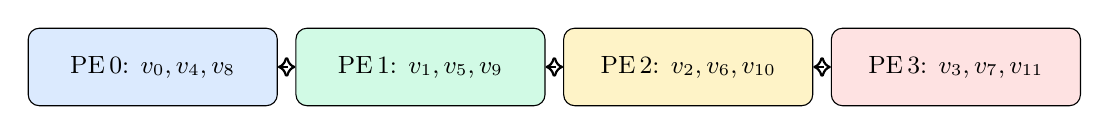
\begin{tikzpicture}[
    pe/.style={draw, rounded corners=4pt, minimum width=90pt, minimum height=28pt, font=\small},
  ]
  \node[pe, fill=pe0color] (pe0) at (0,0) {PE\,0: $v_0, v_4, v_8$};
  \node[pe, fill=pe1color] (pe1) at (3.4,0) {PE\,1: $v_1, v_5, v_9$};
  \node[pe, fill=pe2color] (pe2) at (6.8,0) {PE\,2: $v_2, v_6, v_{10}$};
  \node[pe, fill=pe3color] (pe3) at (10.2,0) {PE\,3: $v_3, v_7, v_{11}$};
  \draw[<->,thick,dashed] (pe0)--(pe1);
  \draw[<->,thick,dashed] (pe1)--(pe2);
  \draw[<->,thick,dashed] (pe2)--(pe3);
\end{tikzpicture}
\end{center}

The hash-based mapping interleaves vertices across PEs instead of assigning contiguous blocks. This spreads high-degree vertices more evenly. Boundary edges may cross multiple PEs: PE\,0$\to$PE\,2 needs one relay through PE\,1; PE\,0$\to$PE\,3 needs two relays. Each relay PE figures out the next hop at runtime using $\texttt{dest\_pe} = \texttt{gid} \mathbin{\&} \texttt{pe\_mask}$---no host-precomputed hop counts needed.

%======================================================================
\section{Stage 4: Compilation and Fabric Wiring}
\label{sec:compilation}
%======================================================================

\subsection{Compilation Command}

The test runner invokes \texttt{cslc} with compile-time parameters that size all PE-local arrays:

\begin{lstlisting}[numbers=none, language=bash, caption={Compilation command for 2-PE layout}]
cslc csl/layout.csl \
  --fabric-dims=10,3 --fabric-offsets=4,1 \
  --memcpy --channels=1 \
  -o csl_compiled_out \
  --params=num_cols:2,num_rows:1,\
    max_local_verts:6,max_local_edges:46,\
    max_boundary:24,max_relay:1,\
    palette_size:16
\end{lstlisting}

\paragraph{Key sizing parameters:}
\begin{itemize}[nosep]
  \item \texttt{max\_local\_verts=6}: the maximum number of vertices any PE holds (used to size \texttt{colors[6]}, \texttt{tentative[6]}, \texttt{csr\_offsets[7]}, etc.)
  \item \texttt{max\_local\_edges=46}: sizes \texttt{csr\_adj[46]}
  \item \texttt{max\_boundary=24}: sizes all three boundary arrays
  \item \texttt{max\_relay=1}: relay buffer depth per direction (for 2 PEs, no relay needed)
  \item \texttt{palette\_size=16}: sizes the \texttt{forbidden[16]} bitmap
\end{itemize}

These are the \emph{max across all PEs across all tests}, so one compiled binary handles any test in the suite.

\subsection{Fabric Layout (\texttt{layout.csl})}

The layout file creates a $\texttt{num\_cols} \times \texttt{num\_rows}$ PE grid and wires 11 fabric colors:

\begin{center}
\renewcommand{\arraystretch}{1.2}
\begin{tabular}{cll}
\toprule
\textbf{Colors} & \textbf{Purpose} & \textbf{Routing} \\
\midrule
C0--C1 & East data wavelets & Checkerboard: even PEs send on C0, odd on C1 \\
C2--C3 & West data wavelets & Same checkerboard, opposite direction \\
C4--C5 & South data (2D only) & Checkerboard vertical \\
C6--C7 & North data (2D only) & Checkerboard vertical \\
C8--C9 & Sync row-reduce (1D) & East$\to$west chain, alternating colors \\
C10    & Sync broadcast (1D)  & West$\to$east from P(0,0) \\
\bottomrule
\end{tabular}
\end{center}

\paragraph{Checkerboard routing.} Adjacent PEs cannot both send on the same fabric color at the same time (hardware rule). The fix: even-column PEs send eastward on C0 and receive on C1; odd-column PEs do the reverse. No two adjacent PEs ever fight for the same wire:

\begin{center}
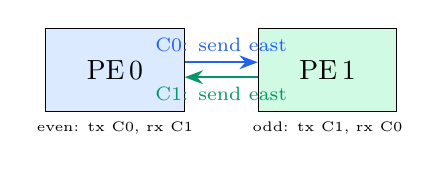
\begin{tikzpicture}[scale=0.9]
  \node[draw, fill=pe0color, minimum width=50pt, minimum height=30pt] (p0) at (0,0) {PE\,0};
  \node[draw, fill=pe1color, minimum width=50pt, minimum height=30pt] (p1) at (3,0) {PE\,1};

  \draw[-{Stealth}, thick, cpuBlue] ([yshift=3pt]p0.east) -- ([yshift=3pt]p1.west)
    node[midway, above, font=\scriptsize] {C0: send east};
  \draw[-{Stealth}, thick, confirmGreen] ([yshift=-3pt]p1.west) -- ([yshift=-3pt]p0.east)
    node[midway, below, font=\scriptsize] {C1: send east};

  \node[font=\tiny, anchor=north] at (0, -0.6) {even: tx C0, rx C1};
  \node[font=\tiny, anchor=north] at (3, -0.6) {odd: tx C1, rx C0};
\end{tikzpicture}
\end{center}

\subsection{Per-PE Code Instantiation}

Each PE tile gets an identical copy of \texttt{pe\_program.csl}, but with unique compile-time parameters:

\begin{lstlisting}[language=CSL, caption={PE instantiation in \texttt{layout.csl} (simplified)}, label=lst:tile]
@set_tile_code(col, row, "pe_program.csl", .{
    .pe_id           = pe_idx,
    .num_cols        = num_cols,
    .is_west_edge    = (col == 0),
    .is_east_edge    = (col == num_cols - 1),
    .send_east_color = if (parity==0) east_color_0 else east_color_1,
    .recv_east_color = if (parity==0) west_color_0 else west_color_1,
    // ... 18 more parameters
});
\end{lstlisting}

Edge flags (\texttt{is\_west\_edge}, \texttt{is\_east\_edge}) let boundary PEs skip sending in directions with no neighbor---a compile-time optimization that removes dead code entirely.

%======================================================================
\section{Stage 5: Host-to-Device Data Transfer}
\label{sec:h2d}
%======================================================================

The host script (\texttt{cerebras\_host.py}) runs inside the Cerebras \texttt{cs\_python} Singularity container. It uses the SDK's \texttt{SdkRuntime} API to upload the partitioned graph.

\subsection{SDK Initialization}

\begin{lstlisting}[language=PyHost, caption={SDK setup (from \texttt{cerebras\_host.py})}, label=lst:sdk]
runner = SdkRuntime(compiled_dir, cmaddr=None)

sym_offsets = runner.get_id('csr_offsets')
sym_adj     = runner.get_id('csr_adj')
sym_colors  = runner.get_id('colors')
sym_nverts  = runner.get_id('local_num_verts')
sym_gids    = runner.get_id('global_vertex_ids')
sym_bnd_local = runner.get_id('boundary_local_idx')
# ... boundary_neighbor_gid, boundary_direction,
#     num_boundary, expected_data_recv, expected_done_recv

runner.load()   # Load compiled binary onto fabric
runner.run()    # Start memcpy infrastructure
\end{lstlisting}

Each \texttt{get\_id()} call resolves a symbol name (matching \texttt{@export\_name} in \texttt{layout.csl}) to a handle used for memory transfers.

\subsection{Per-PE Upload Loop}

For each PE, the host pads arrays to \texttt{max\_local\_verts}/\texttt{max\_local\_edges}/\texttt{max\_boundary} (required by the fixed compile-time array sizes) and transfers them:

\begin{lstlisting}[language=PyHost, caption={Uploading to one PE (from \texttt{cerebras\_host.py})}, label=lst:h2d]
for pe_idx in range(total_pes):
    pe_col = pe_idx % num_cols
    pe_row = pe_idx // num_cols
    d = graph_data[pe_idx]

    # Pad to compile-time max sizes
    off_padded = np.zeros(max_local_verts + 1, dtype=np.int32)
    off_padded[:len(d['local_offsets'])] = d['local_offsets']

    adj_padded = np.zeros(max_local_edges, dtype=np.int32)
    adj_padded[:len(d['local_adj'])] = d['local_adj']

    # Transfer via memcpy (DMA through fabric)
    runner.memcpy_h2d(sym_offsets, off_padded,
                      pe_col, pe_row, 1, 1,
                      max_local_verts + 1, streaming=False,
                      data_type=MemcpyDataType.MEMCPY_32BIT,
                      nonblock=False)
    # ... repeat for adj, colors, gids, boundary arrays
\end{lstlisting}

\paragraph{Transfer breakdown for our 2-PE example:}

\begin{center}
\renewcommand{\arraystretch}{1.2}
\begin{tabular}{lrrl}
\toprule
\textbf{Symbol} & \textbf{Words/PE} & \textbf{$\times$ 2 PEs} & \textbf{Total} \\
\midrule
\texttt{csr\_offsets}     & 7    & 14   & 56 B \\
\texttt{csr\_adj}         & 46   & 92   & 368 B \\
\texttt{colors}           & 6    & 12   & 48 B \\
\texttt{local\_num\_verts} & 1   & 2    & 8 B \\
\texttt{global\_vertex\_ids} & 6 & 12   & 48 B \\
\texttt{boundary\_local\_idx} & 24 & 48 & 192 B \\
\texttt{boundary\_neighbor\_gid} & 24 & 48 & 192 B \\
\texttt{boundary\_direction} & 24 & 48 & 192 B \\
\texttt{num\_boundary}    & 1    & 2    & 8 B \\
\texttt{pe\_mask}         & 1    & 2    & 8 B \\
\texttt{expected\_data\_recv} & 1 & 2 & 8 B \\
\texttt{expected\_done\_recv} & 1 & 2 & 8 B \\
\midrule
\textbf{Total uploaded}   &      &      & \textbf{1,136 B} \\
\bottomrule
\end{tabular}
\end{center}

\subsection{Launch}

After all data is uploaded, one host call launches the kernel on every PE at once:

\begin{lstlisting}[language=PyHost, numbers=none]
runner.launch('start_coloring', nonblock=False)
\end{lstlisting}

This resolves to \texttt{start\_coloring()} exported from \texttt{pe\_program.csl}. From this point on, \textbf{no host involvement occurs} until all rounds finish---the PEs run entirely on their own.

%======================================================================
\section{Stage 6: On-Fabric Execution --- The PE Kernel}
\label{sec:kernel}
%======================================================================

This is the heart of the whole system. Every PE runs the same task-driven program, chained in a BSP loop: Speculate $\to$ Send $\to$ Recv $\to$ Barrier $\to$ Detect/Resolve $\to$ (loop or converge). There is no fixed round limit; the algorithm keeps going until \textbf{global convergence} is detected through an OR-reduce piggybacked on the barrier (Section~\ref{sec:convergence}).

\begin{center}
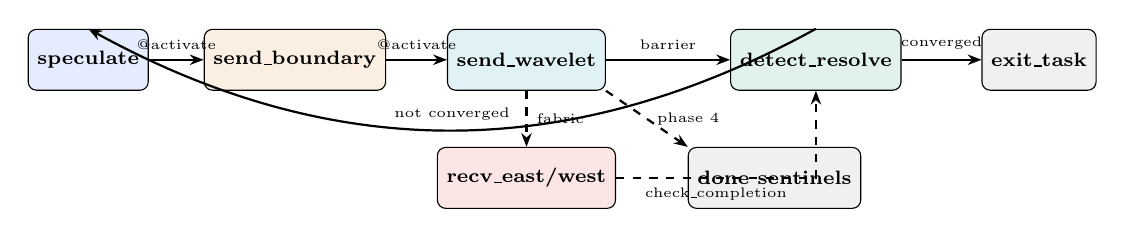
\begin{tikzpicture}[
    task/.style={draw, rounded corners=3pt, minimum height=22pt, font=\scriptsize\bfseries, fill=#1!12},
    arrow/.style={-{Stealth[length=5pt]}, thick},
    xscale=1.05
  ]
  \node[task=cpuBlue]      (S) at (0, 0)   {speculate};
  \node[task=warnOrange]   (B) at (2.5, 0) {send\_boundary};
  \node[task=wseColor]     (W) at (5.3, 0) {send\_wavelet};
  \node[task=conflictRed]  (R) at (5.3, -1.5) {recv\_east/west};
  \node[task=gray]         (DN) at (8.3, -1.5) {done sentinels};
  \node[task=confirmGreen] (D) at (8.8, 0) {detect\_resolve};
  \node[task=gray]         (X) at (11.5, 0) {exit\_task};

  \draw[arrow] (S) -- (B) node[midway, above, font=\tiny] {@activate};
  \draw[arrow] (B) -- (W) node[midway, above, font=\tiny] {@activate};
  \draw[arrow, dashed] (W.south) -- (R.north) node[midway, right, font=\tiny] {fabric};
  \draw[arrow] (W) -- (D) node[midway, above, font=\tiny] {barrier};
  \draw[arrow, dashed] (W.south east) -- (DN.north west) node[midway, right, font=\tiny] {phase 4};
  \draw[arrow, dashed] (R.east) -| (D.south) node[near start, below, font=\tiny] {check\_completion};
  \draw[arrow] (D) -- (X) node[midway, above, font=\tiny] {converged};
  \draw[arrow, bend left=30] (D.north) to node[above, font=\tiny] {not converged} (S.north);
\end{tikzpicture}
\end{center}

\subsection{Entry Point: \texttt{start\_coloring()}}

\begin{lstlisting}[language=CSL, caption={Entry point (from \texttt{pe\_program.csl})}, label=lst:entry]
fn start_coloring() void {
    start_timing();       // enable hardware TSC counter

    // Initialize remote color buffer to "unknown"
    var b: i16 = 0;
    while (b < max_boundary) : (b += 1) {
        remote_recv_color[b] = -1;
    }
    current_round = 0;
    data_recv_remaining = expected_data_recv[0];
    done_recv_count = 0;   // done sentinels received this round
    // ... reset all state flags (local_send_done, phase_complete, etc.) ...

    @activate(speculate_task_id);  // kick off first round
}
\end{lstlisting}

\subsection{Phase 1: Speculate}

Each PE iterates over its local vertices and assigns the smallest available color:

\begin{lstlisting}[language=CSL, caption={Speculate task (simplified from \texttt{pe\_program.csl})}, label=lst:spec]
task speculate() void {
    const n = local_num_verts[0];
    var v: i16 = 0;
    while (v < max_local_verts) : (v += 1) {
        if (v >= n) break;
        if (colors[v] >= 0) continue;  // already colored

        // Build forbidden set from ALL neighbors
        // (local: direct lookup, remote: from last round's wavelets)
        var c: i16 = 0;
        while (c < palette_size) : (c += 1) { forbidden[c] = 0; }

        const start = csr_offsets[v];
        const end_idx = csr_offsets[v + 1];
        var e: i32 = start;
        while (e < end_idx) : (e += 1) {
            const neighbor_gid = csr_adj[e];
            const local_idx = global_to_local(neighbor_gid);
            if (local_idx >= 0) {
                // Local neighbor: read directly
                const nc = colors[local_idx];
                if (nc >= 0) forbidden[nc] = 1;
            } else {
                // Remote neighbor: check last round's wavelet data
                // (stored in remote_recv_color[])
                // ... scan boundary table for matching GID ...
            }
        }
        tentative[v] = find_min_available_color();
        if (tentative[v] >= 0) colors[v] = tentative[v];
    }

    // Local conflict check: higher GID yields
    // ... scan local edges for tentative[v] == tentative[w] ...

    @activate(send_boundary_task_id);
}
\end{lstlisting}

\paragraph{Round 1 trace for PE\,0 (2-PE layout):}

With hash partitioning, PE\,0 holds $\{v_0, v_2, v_4, v_6, v_8, v_{10}\}$. Since \texttt{colors[v]} is set immediately during the forward scan, later vertices see colors assigned to earlier local vertices in the same speculate call:

\begin{center}
\renewcommand{\arraystretch}{1.3}
\begin{tabular}{llll}
\toprule
\textbf{Vertex} & \textbf{Forbidden (from local neighbors)} & \textbf{Chosen} & \textbf{Notes} \\
\midrule
$v_0$ & $\{\}$ (local nbrs $v_4,v_6,v_8,v_{10}$ uncolored) & color 0 & First available \\
$v_2$ & $\{\}$ (local nbrs $v_4,v_6,v_8,v_{10}$ uncolored; $v_0$ not adjacent) & color 0 & $v_0 \notin \mathrm{adj}(v_2)$ \\
$v_4$ & $\{0\}$ ($v_0{=}0, v_2{=}0$ are local nbrs) & color 1 & Avoids 0 \\
$v_6$ & $\{0,1\}$ ($v_0{=}0, v_2{=}0, v_4{=}1$) & color 2 & \\
$v_8$ & $\{0,1\}$ ($v_0{=}0, v_2{=}0, v_4{=}1$) & color 2 & Same as $v_6$ \\
$v_{10}$ & $\{0,1\}$ ($v_0{=}0, v_2{=}0, v_4{=}1$) & color 2 & Same again \\
\bottomrule
\end{tabular}
\end{center}

\paragraph{Local conflict check:}
\begin{itemize}[nosep]
  \item $v_0{=}0$ vs $v_2{=}0$: \textbf{not adjacent}---$v_0$ and $v_2$ are not in each other's neighbor lists, so no conflict
  \item $v_6{=}2, v_8{=}2, v_{10}{=}2$: pairwise \textbf{not adjacent}---no conflicts
\end{itemize}

After local conflict resolution: \textbf{PE\,0 keeps all 6 colors}---$v_0{=}0, v_2{=}0, v_4{=}1, v_6{=}2, v_8{=}2, v_{10}{=}2$.

\subsection{Phase 2: Send Boundary Wavelets}

\subsubsection{Wavelet Format}

Each wavelet is a single 32-bit word packing the sender GID, destination PE, and color into a compact encoding. Two compile-time modes exist, selected by the \texttt{use\_hw\_filter} flag:

\begin{center}
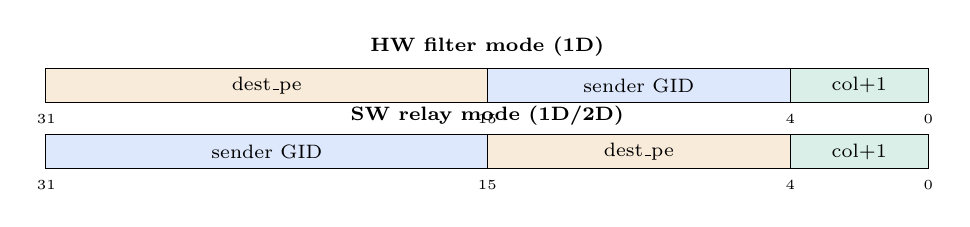
\begin{tikzpicture}[scale=0.35]
  % HW filter mode
  \node[font=\scriptsize\bfseries, anchor=south] at (16, 2.8) {HW filter mode (1D)};
  \draw[thick] (0,1.5) rectangle (32,2.7);
  \fill[warnOrange!15] (0,1.5) rectangle (16,2.7);
  \fill[cpuBlue!15] (16,1.5) rectangle (27,2.7);
  \fill[confirmGreen!15] (27,1.5) rectangle (32,2.7);
  \draw (16,1.5)--(16,2.7);
  \draw (27,1.5)--(27,2.7);
  \node[font=\scriptsize] at (8, 2.1) {dest\_pe};
  \node[font=\scriptsize] at (21.5, 2.1) {sender GID};
  \node[font=\scriptsize] at (29.5, 2.1) {col+1};
  \node[font=\tiny, anchor=north] at (0, 1.4) {31};
  \node[font=\tiny, anchor=north] at (16, 1.4) {15};
  \node[font=\tiny, anchor=north] at (27, 1.4) {4};
  \node[font=\tiny, anchor=north] at (32, 1.4) {0};

  % SW relay mode
  \node[font=\scriptsize\bfseries, anchor=south] at (16, 0.3) {SW relay mode (1D/2D)};
  \draw[thick] (0,-0.9) rectangle (32,0.3);
  \fill[cpuBlue!15] (0,-0.9) rectangle (16,0.3);
  \fill[warnOrange!15] (16,-0.9) rectangle (27,0.3);
  \fill[confirmGreen!15] (27,-0.9) rectangle (32,0.3);
  \draw (16,-0.9)--(16,0.3);
  \draw (27,-0.9)--(27,0.3);
  \node[font=\scriptsize] at (8, -0.3) {sender GID};
  \node[font=\scriptsize] at (21.5, -0.3) {dest\_pe};
  \node[font=\scriptsize] at (29.5, -0.3) {col+1};
  \node[font=\tiny, anchor=north] at (0, -1.0) {31};
  \node[font=\tiny, anchor=north] at (16, -1.0) {15};
  \node[font=\tiny, anchor=north] at (27, -1.0) {4};
  \node[font=\tiny, anchor=north] at (32, -1.0) {0};
\end{tikzpicture}
\end{center}

\begin{lstlisting}[language=CSL, caption={Wavelet packing (from \texttt{pe\_program.csl})}, label=lst:pack]
fn pack_wavelet(gid: i32, dest_pe: i32, col: i32) u32 {
  if (use_hw_filter) {
    // HW filter: dest_pe in upper 16 (filter key)
    const upper    = @as(u32, @as(u16, @as(i16, dest_pe))) << 16;
    const gid_part = (@as(u32, @as(u16, @as(i16, gid))) & 0x7FF) << 5;
    const col_part = @as(u32, @as(u16, @as(i16, col + 1))) & 0x1F;
    return upper | gid_part | col_part;
  } else {
    // SW relay: sender_gid in upper 16, dest_pe in [15:5], color in [4:0]
    const id_part  = @as(u32, @as(u16, @as(i16, gid)));
    const dpe_part = (@as(u32, @as(u16, @as(i16, dest_pe))) & 0x7FF) << 5;
    const col_part = @as(u32, @as(u16, @as(i16, col + 1))) & 0x1F;
    return (id_part << 16) | dpe_part | col_part;
  }
}
\end{lstlisting}

In both modes, the color is stored as $c + 1$ so that color~0 maps to value~1, leaving value~0 free to mean ``uncolored.'' Done sentinels use $\texttt{color} = -1$, which encodes as $-1+1 = 0$ in the 5-bit color field---this lets us multiplex data and control signals in the same wavelet format with zero overhead.

\subsubsection{Cooperative Send Chain}

Boundary wavelets are sent \textbf{one per task activation} to avoid output FIFO deadlock. Between sends, receive data tasks can fire and drain input FIFOs:

\begin{lstlisting}[language=CSL, caption={One-at-a-time send (from \texttt{pe\_program.csl})}, label=lst:sendchain]
task send_wavelet() void {
    // Priority: drain one relay wavelet first
    if (drain_one_relay()) {
        @activate(send_wavelet_task_id);
        return;
    }
    // Phase 0: east sends
    if (send_phase == 0) {
        if (!is_east_edge and send_idx < east_count) {
            send_wavelet_east(east_send_buf[send_idx]);
            send_idx += 1;
            @activate(send_wavelet_task_id);
            return;
        }
        send_phase = 1; send_idx = 0;
    }
    // Phase 1: west sends ... Phase 2: south ... Phase 3: north
    // Phase 4: done sentinels (one per unique destination PE)
    if (send_phase == 4) {
        if (send_idx < done_send_count) {
            const dir = done_send_dir[send_idx];
            const wval = done_send_buf[send_idx];
            if      (dir == 0) send_wavelet_east(wval);
            else if (dir == 1) send_wavelet_west(wval);
            // ... south, north for 2D
            send_idx += 1;
            @activate(send_wavelet_task_id);
            return;
        }
        send_phase = 5; send_idx = 0;
    }
    // Phase 5: final relay drain + completion check
}
\end{lstlisting}

\subsubsection{Completion Detection}

The host precomputes \texttt{expected\_data\_recv} (the total number of data wavelets each PE should receive) and \texttt{expected\_done\_recv} (the number of unique source PEs sending to it), both uploaded alongside the graph data. Each receive handler decrements \texttt{data\_recv\_remaining}; done sentinels increment \texttt{done\_recv\_count}. Completion uses a dual-path check:

\begin{lstlisting}[language=CSL, numbers=none, caption={Dual-path completion (from \texttt{pe\_program.csl})}]
// Host-precomputed: uploaded via H2D
var expected_data_recv: [1]i32;      // total data wavelets to expect
var expected_done_recv: [1]i32;      // unique source PEs sending to us
var data_recv_remaining: i32 = 0;
var done_recv_count: i32 = 0;

fn check_completion() void {
    if (!phase_complete and local_send_done and all_relay_drained()) {
        if (data_recv_remaining <= 0) {
            // Normal path: all expected data received
            phase_complete = true;
            on_data_complete();
        } else if (done_recv_count >= expected_done_recv[0]) {
            // Overflow recovery: all senders finished, but some
            // data was lost to relay buffer overflow. Proceed
            // anyway so the algorithm doesn't hang forever.
            phase_complete = true;
            on_data_complete();
        }
    }
}
\end{lstlisting}

Two paths reach completion. The \textbf{normal path} fires when \texttt{data\_recv\_remaining} reaches zero---every expected wavelet arrived. The \textbf{overflow recovery path} fires when every source PE has sent a done sentinel (\texttt{done\_recv\_count $\geq$ expected\_done\_recv}), meaning all senders have finished even though some relay wavelets were dropped. Without the second path, a PE waiting for lost wavelets would hang forever.

\subsection{Phase 3: Receive and Relay}

Receive handlers fire as hardware data tasks whenever a wavelet shows up on the PE's input queue. The handler is a thin wrapper around \texttt{route\_data\_wavelet()}, which inspects \texttt{dest\_pe} to decide whether to consume or relay:

\begin{lstlisting}[language=CSL, caption={East receive handler (from \texttt{pe\_program.csl})}, label=lst:recv]
task recv_east(wval: u32) void {
    route_data_wavelet(wval);
    check_completion();
}

fn route_data_wavelet(wval: u32) void {
    const dest_pe = unpack_dest_pe(wval);
    if (dest_pe == @as(i32, pe_id)) {
        const recv_col = unpack_color(wval);
        if (recv_col < 0) {
            // Done sentinel: sender finished all its sends
            done_recv_count += 1;
        } else {
            // Normal data wavelet
            process_incoming_wavelet(
                unpack_gid(wval), recv_col);
            data_recv_remaining -= 1;
        }
    } else if (num_rows == 1) {
        // 1D: relay east or west based on dest_pe
        if (dest_pe > @as(i32, pe_id)) buffer_relay_east(wval);
        else                            buffer_relay_west(wval);
    } else {
        // 2D: Manhattan horizontal-first routing
    }
}
\end{lstlisting}

\texttt{process\_incoming\_wavelet()} stores the received color in \texttt{remote\_recv\_color[b]} for every matching boundary entry:

\begin{lstlisting}[language=CSL, numbers=none]
fn process_incoming_wavelet(sender_gid: i32, sender_color: i32) void {
    const nbnd = num_boundary[0];
    var b: i16 = 0;
    while (b < max_boundary) : (b += 1) {
        if (@as(i32, b) >= nbnd) break;
        if (boundary_neighbor_gid[b] == sender_gid) {
            remote_recv_color[b] = sender_color;
        }
    }
}
\end{lstlisting}

\subsection{Global Barrier with Convergence Detection}
\label{sec:convergence}

Before detect/resolve can run, \textbf{every PE must have finished sending and receiving}. In 1D mode, we use a two-phase hardware barrier that also carries convergence info via an OR-reduce:

\begin{enumerate}[nosep]
  \item \textbf{Row-reduce with OR} (east$\to$west): The easternmost PE sends a sync wavelet west. The wavelet payload is \texttt{sync\_buf[0]}, which each PE sets to~1 if it has \emph{any} uncolored vertices, or~0 if all local vertices are colored. As each PE forwards the reduce signal west, it \textbf{ORs} the incoming value with its own: \texttt{sync\_buf[0] = sync\_buf[0] | wval}. When P(0,0) receives the reduced value, it holds the global OR---1 if \emph{any} PE still has uncolored vertices.
  \item \textbf{Broadcast} (P(0,0)$\to$all east): P(0,0) sends the reduced value eastward as a broadcast wavelet. Each PE stores this global result.
  \item \textbf{Convergence check}: When a PE completes the barrier (both data received and broadcast received), it checks: if \texttt{current\_round > 0} and the reduced value is~0 (no PE has uncolored vertices), the algorithm has \textbf{converged} and the PE jumps directly to \texttt{exit\_task}. Otherwise it proceeds to \texttt{detect\_resolve}.
\end{enumerate}

\begin{center}
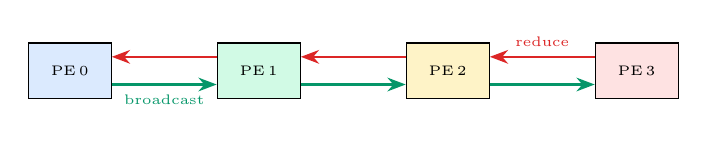
\begin{tikzpicture}[xscale=1.2]
  \node[draw, fill=pe0color, minimum width=30pt, minimum height=20pt, font=\tiny] (p0) at (0,0) {PE\,0};
  \node[draw, fill=pe1color, minimum width=30pt, minimum height=20pt, font=\tiny] (p1) at (2,0) {PE\,1};
  \node[draw, fill=pe2color, minimum width=30pt, minimum height=20pt, font=\tiny] (p2) at (4,0) {PE\,2};
  \node[draw, fill=pe3color, minimum width=30pt, minimum height=20pt, font=\tiny] (p3) at (6,0) {PE\,3};

  % Row reduce
  \draw[-{Stealth}, conflictRed, thick] ([yshift=5pt]p3.west) -- ([yshift=5pt]p2.east) node[midway, above, font=\tiny] {reduce};
  \draw[-{Stealth}, conflictRed, thick] ([yshift=5pt]p2.west) -- ([yshift=5pt]p1.east);
  \draw[-{Stealth}, conflictRed, thick] ([yshift=5pt]p1.west) -- ([yshift=5pt]p0.east);

  % Broadcast
  \draw[-{Stealth}, confirmGreen, thick] ([yshift=-5pt]p0.east) -- ([yshift=-5pt]p1.west) node[midway, below, font=\tiny] {broadcast};
  \draw[-{Stealth}, confirmGreen, thick] ([yshift=-5pt]p1.east) -- ([yshift=-5pt]p2.west);
  \draw[-{Stealth}, confirmGreen, thick] ([yshift=-5pt]p2.east) -- ([yshift=-5pt]p3.west);
\end{tikzpicture}
\end{center}

A PE only sends its reduce signal \textbf{after} \texttt{on\_data\_complete()} fires (meaning all data wavelets have been received). So the reduce signal only ever propagates through PEs that are truly done.

\subsubsection{Barrier Correctness: Blocked Task Gating}

There is a subtle but important invariant that makes this barrier correct: the \texttt{sync\_reduce\_task} starts \textbf{blocked} at compile time and only gets unblocked inside \texttt{on\_data\_complete()}. The reduce chain physically \emph{cannot} propagate through a PE until that PE has finished its own data exchange:

\begin{lstlisting}[language=CSL, numbers=none, caption={Sync tasks start blocked (from \texttt{pe\_program.csl})}]
comptime {
    @bind_data_task(sync_reduce_recv, sync_reduce_task_id);
    @bind_data_task(sync_bcast_recv, sync_bcast_task_id);
    @block(sync_reduce_task_id);   // blocked at init
    @block(sync_bcast_task_id);    // blocked at init
}
\end{lstlisting}

\begin{lstlisting}[language=CSL, numbers=none, caption={Unblock only when data exchange is complete}]
fn on_data_complete() void {
    local_data_done = true;
    if (is_east_edge) {
        send_sync_reduce();            // east PE initiates chain
        @unblock(sync_bcast_task_id);  // arm for broadcast
    } else {
        @unblock(sync_reduce_task_id); // arm for reduce from east
    }
    maybe_proceed();
}
\end{lstlisting}

Consider a 4-PE example where PE\,3 (eastmost) finishes data exchange first and sends the reduce wavelet west. If PE\,2 is still receiving data wavelets:

\begin{enumerate}[nosep]
  \item PE\,3's reduce wavelet arrives at PE\,2's input queue for \texttt{sync\_reduce\_recv\_color}
  \item PE\,2's \texttt{sync\_reduce\_task} is still \textbf{blocked} $\Rightarrow$ the wavelet \emph{sits in the queue without being processed}
  \item PE\,2 eventually completes data exchange $\Rightarrow$ \texttt{on\_data\_complete()} calls \texttt{@unblock(sync\_reduce\_task\_id)}
  \item \emph{Now} PE\,2's reduce task fires: it OR-combines and forwards the wavelet westward to PE\,1
  \item The same gating mechanism applies at PE\,1 and PE\,0
\end{enumerate}

The broadcast from P(0,0) cannot be sent until P(0,0) receives the completed reduce chain, which requires \emph{every} intermediate PE to have finished and unblocked. Therefore:

\begin{center}
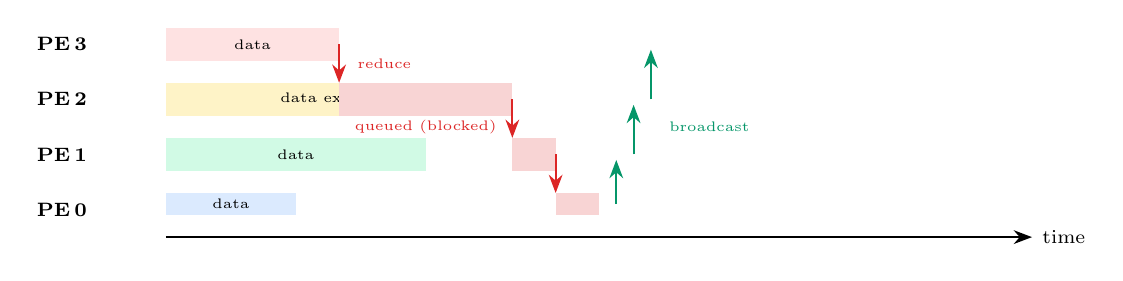
\begin{tikzpicture}[xscale=1.1, yscale=0.7]
  \node[font=\scriptsize\bfseries] at (-1.2, 3) {PE\,3};
  \node[font=\scriptsize\bfseries] at (-1.2, 2) {PE\,2};
  \node[font=\scriptsize\bfseries] at (-1.2, 1) {PE\,1};
  \node[font=\scriptsize\bfseries] at (-1.2, 0) {PE\,0};

  % Time axis
  \draw[-{Stealth}, thick] (0, -0.5) -- (10, -0.5) node[right, font=\scriptsize] {time};

  % PE 3: finishes early
  \fill[pe3color] (0,2.7) rectangle (2,3.3);
  \node[font=\tiny] at (1, 3) {data};
  \draw[-{Stealth}, conflictRed, thick] (2, 3) -- (2, 2.3);
  \node[font=\tiny, conflictRed, anchor=west] at (2.1, 2.65) {reduce};

  % PE 2: still busy, reduce waits
  \fill[pe2color] (0,1.7) rectangle (4,2.3);
  \node[font=\tiny] at (2, 2) {data exchange};
  \fill[conflictRed!20] (2,1.7) rectangle (4,2.3);
  \node[font=\tiny, conflictRed] at (3, 1.5) {queued (blocked)};
  \draw[-{Stealth}, conflictRed, thick] (4, 2) -- (4, 1.3);

  % PE 1: finishes after PE 2
  \fill[pe1color] (0,0.7) rectangle (3,1.3);
  \node[font=\tiny] at (1.5, 1) {data};
  \fill[conflictRed!20] (4,0.7) rectangle (4.5,1.3);
  \draw[-{Stealth}, conflictRed, thick] (4.5, 1) -- (4.5, 0.3);

  % PE 0: receives reduce, sends broadcast
  \fill[pe0color] (0,-0.1) rectangle (1.5,0.3);
  \node[font=\tiny] at (0.75, 0.1) {data};
  \fill[conflictRed!20] (4.5,-0.1) rectangle (5,0.3);
  \draw[-{Stealth}, confirmGreen, thick] (5.2, 0.1) -- (5.2, 0.9);
  \draw[-{Stealth}, confirmGreen, thick] (5.4, 1) -- (5.4, 1.9);
  \draw[-{Stealth}, confirmGreen, thick] (5.6, 2) -- (5.6, 2.9);
  \node[font=\tiny, confirmGreen, anchor=west] at (5.7, 1.5) {broadcast};
\end{tikzpicture}
\end{center}

\textbf{No PE can enter \texttt{detect\_resolve} until every PE has completed data exchange.} The blocked task mechanism gives us a hardware-enforced gate that makes this guarantee without any polling or busy-waiting.

\subsubsection{Round Boundary Safety}

After the barrier, PEs enter \texttt{detect\_resolve} and then \texttt{speculate} at slightly different times. This is safe because:

\begin{enumerate}[nosep]
  \item \texttt{maybe\_proceed()} calls \texttt{block\_all\_recv()} \emph{before} activating \texttt{detect\_resolve}---closing the receive window
  \item Recv stays blocked through \texttt{detect\_resolve} $\to$ \texttt{speculate}
  \item Only \texttt{send\_boundary()} calls \texttt{unblock\_all\_recv()}---\emph{after} resetting \texttt{data\_recv\_remaining}
  \item The sync barrier tasks are re-blocked inside their own handlers (\texttt{@block(sync\_reduce\_task\_id)})
\end{enumerate}

Even if a fast PE starts sending round $N{+}1$ wavelets before a slow PE has entered \texttt{detect\_resolve} for round $N$, no problem: the slow PE's receive tasks are blocked, so wavelets just queue up harmlessly in the hardware input FIFOs until the PE is ready.

The convergence check in \texttt{maybe\_proceed()} is:

\begin{lstlisting}[language=CSL, caption={Convergence-aware barrier completion}, label=lst:converge]
fn maybe_proceed() void {
    if (local_data_done and sync_barrier_done) {
        // sync_buf[0] holds the global OR-reduced
        // "has_uncolored" flag after the barrier.
        if (current_round > 0 and sync_buf[0] == 0) {
            @activate(exit_task_id);  // converged!
        } else {
            @activate(detect_resolve_task_id);
        }
    }
}
\end{lstlisting}

The OR-reduce in the sync receive handler:

\begin{lstlisting}[language=CSL, caption={OR-reduce in barrier receive}, label=lst:orreduce]
task sync_reduce_recv(wval: u32) void {
    @block(sync_reduce_task_id);
    sync_buf[0] = sync_buf[0] | wval;  // OR-reduce
    if (is_west_edge) {
        send_sync_bcast();            // broadcast reduced value
        sync_barrier_done = true;
        maybe_proceed();
    } else {
        send_sync_reduce();           // forward west
        @unblock(sync_bcast_task_id); // wait for broadcast
    }
}
\end{lstlisting}

So there is \textbf{no fixed round limit}. The algorithm terminates when every PE's local vertices are colored and no conflicts remain. In practice, the 12-node test converges in just \textbf{3 rounds} (one productive round + one conflict-resolution round + one verification round).

\subsection{Phase 4: Detect and Resolve Boundary Conflicts}

\begin{lstlisting}[language=CSL, caption={Detect/resolve with convergence tracking (from \texttt{pe\_program.csl})}, label=lst:detect]
task detect_resolve() void {
    const nbnd = num_boundary[0];
    var had_conflict: bool = false;
    var b: i16 = 0;
    while (b < max_boundary) : (b += 1) {
        if (b >= nbnd) break;
        const li = boundary_local_idx[b];
        const my_gid = global_vertex_ids[li];
        const nbr_gid = boundary_neighbor_gid[b];
        const my_color = colors[li];
        const remote_color = remote_recv_color[b];
        if (my_color >= 0 and remote_color >= 0
            and my_color == remote_color) {
            if (my_gid > nbr_gid) {
                colors[li] = -1;   // yield: revert to uncolored
                had_conflict = true;
            }
        }
    }
    // Check if any local vertex is still uncolored
    var has_uncolored: bool = had_conflict;
    if (!has_uncolored) {
        const n = local_num_verts[0];
        var v: i16 = 0;
        while (v < max_local_verts) : (v += 1) {
            if (v >= n) break;
            if (colors[v] < 0) { has_uncolored = true; break; }
        }
    }
    // Store in sync_buf for next round's barrier OR-reduce
    sync_buf[0] = if (has_uncolored) 1 else 0;

    current_round += 1;
    // Reset state and start next round (convergence is
    // detected by the barrier, not by a round counter)
    data_recv_remaining = expected_data_recv[0];  // count-based reset
    done_recv_count = 0;                          // sentinel reset
    // ... reset all relay/sync flags ...
    @activate(speculate_task_id);  // next round
}
\end{lstlisting}

There is no \texttt{max\_rounds} check. After each \texttt{detect\_resolve}, the PE records whether it still has uncolored vertices in \texttt{sync\_buf[0]}, then starts the next round unconditionally. The \emph{barrier} in the next round reads \texttt{sync\_buf[0]} via the OR-reduce; if the global OR is~0 (nobody has uncolored vertices), \texttt{maybe\_proceed()} terminates the algorithm before \texttt{detect\_resolve} even runs.

\subsection{Round-by-Round Trace (2 PEs)}

\paragraph{Round 1:}
\begin{center}
\renewcommand{\arraystretch}{1.2}
\begin{tabular}{llll}
\toprule
& \textbf{After Speculate} & \textbf{After Local Conflict} & \textbf{After Boundary Resolve} \\
\midrule
PE\,0 & $v_0{=}0, v_2{=}0, v_4{=}1, v_6{=}2, v_8{=}2, v_{10}{=}2$ & all kept (no local conflicts) & all kept \\
PE\,1 & $v_1{=}0, v_3{=}1, v_5{=}1, v_7{=}2, v_9{=}1, v_{11}{=}3$ & all kept (no local conflicts) & $v_7, v_9$ yield \\
\bottomrule
\end{tabular}
\end{center}

After round 1: 10 vertices colored, 2 remain ($v_7, v_9$ on PE\,1). The boundary conflicts are $v_7{=}2$ vs $v_6{=}2$ (GID $7 > 6$, $v_7$ yields) and $v_9{=}1$ vs $v_4{=}1$ (GID $9 > 4$, $v_9$ yields).

\paragraph{Round 2:}
$v_7$ now sees $\{v_1{=}0, v_3{=}1, v_{11}{=}3\}$ (local) and $\{v_0{=}0, v_2{=}0, v_6{=}2\}$ (from wavelets) $\Rightarrow$ forbidden $= \{0,1,2,3\}$, picks color~4. $v_9$ sees $\{v_1{=}0, v_7{=}4, v_{11}{=}3\}$ and $\{v_0{=}0, v_2{=}0, v_4{=}1, v_8{=}2\}$ $\Rightarrow$ forbidden $= \{0,1,2,3,4\}$, picks color~5. No conflicts remain.

The process converges after \textbf{3 rounds} (the third round is a verification round where the barrier's OR-reduce confirms global convergence), using \textbf{6 colors}.

%======================================================================
\section{Stage 7: Device-to-Host Result Retrieval}
\label{sec:d2h}
%======================================================================

\subsection{Reading Colors}

After \texttt{launch()} returns (all PEs have called \texttt{sys\_mod.unblock\_cmd\_stream()}), the host reads back each PE's colors:

\begin{lstlisting}[language=PyHost, caption={Color readback (from \texttt{cerebras\_host.py})}, label=lst:d2h]
all_colors = np.full(num_verts, -1, dtype=np.int32)
for pe_idx in range(total_pes):
    pe_col = pe_idx % num_cols
    pe_row = pe_idx // num_cols
    d = graph_data[pe_idx]
    local_n = d['local_n']
    buf = np.zeros(max_local_verts, dtype=np.int32)
    runner.memcpy_d2h(buf, sym_colors,
                      pe_col, pe_row, 1, 1,
                      max_local_verts, streaming=False,
                      data_type=MemcpyDataType.MEMCPY_32BIT)
    # Hash-based: use the global_ids list to map back
    for i in range(local_n):
        gid = d['global_ids'][i]
        all_colors[gid] = buf[i]
\end{lstlisting}

Colors are reassembled into a global array using each PE's \texttt{global\_ids} list to map local indices back to global vertex IDs. This mapping is necessary because hash-based partitioning does not give each PE a contiguous range of vertices.

\subsection{Hardware Cycle Counter Readback}

Each PE records start and end timestamps using the WSE hardware TSC (Timestamp Counter). The \texttt{<time>} CSL module gives us an always-running cycle counter with sub-cycle precision:

\begin{lstlisting}[language=CSL, caption={TSC timing (from \texttt{pe\_program.csl})}, label=lst:tsc]
const tsc = @import_module("<time>");
var tsc_start_buf = @zeros([tsc.tsc_size_words]u16);
var tsc_end_buf   = @zeros([tsc.tsc_size_words]u16);
var coloring_timer = @zeros([3]f32);

inline fn start_timing() void {
    tsc.enable_tsc();
    tsc.get_timestamp(&tsc_start_buf);
}

inline fn stop_timing() void {
    tsc.get_timestamp(&tsc_end_buf);
    tsc.disable_tsc();

    // Pack 6 x u16 timestamps into 3 x f32 for host readback
    var lo_: u16 = 0; var hi_: u16 = 0;
    lo_ = tsc_start_buf[0]; hi_ = tsc_start_buf[1];
    coloring_timer[0] = @bitcast(f32, (@as(u32, hi_) << @as(u16, 16)) | @as(u32, lo_));
    lo_ = tsc_start_buf[2]; hi_ = tsc_end_buf[0];
    coloring_timer[1] = @bitcast(f32, (@as(u32, hi_) << @as(u16, 16)) | @as(u32, lo_));
    lo_ = tsc_end_buf[1]; hi_ = tsc_end_buf[2];
    coloring_timer[2] = @bitcast(f32, (@as(u32, hi_) << @as(u16, 16)) | @as(u32, lo_));
}
\end{lstlisting}

The host reads the packed timer data and converts to cycles:

\begin{lstlisting}[language=PyHost, caption={Cycle count computation (from \texttt{cerebras\_host.py})}, label=lst:cycles]
from cerebras.sdk.sdk_utils import calculate_cycles

timing_data = np.zeros(num_rows * num_cols * 3, dtype=np.uint32)
runner.memcpy_d2h(timing_data, sym_timer, 0, 0,
                  num_cols, num_rows, 3, ...)
timing_hwl = timing_data.view(np.float32).reshape(
    (num_rows, num_cols, 3))

max_cycles = 0
for pe_row in range(num_rows):
    for pe_col in range(num_cols):
        cycles = calculate_cycles(
            timing_hwl[pe_row, pe_col, :])
        max_cycles = max(max_cycles, int(cycles))

elapsed_ms = (max_cycles / 850_000_000) * 1000
\end{lstlisting}

The wall-clock time is the \textbf{maximum} across all PEs---the slowest PE sets the total time since the algorithm is synchronous.

%======================================================================
\section{Stage 8: Validation}
\label{sec:validation}
%======================================================================

The test runner checks two things:

\subsection{Correctness: No Adjacent Vertices Share a Color}

\begin{lstlisting}[language=Python, caption={Validation (from \texttt{run\_csl\_tests.py})}, label=lst:validate]
def validate_coloring(num_verts, edges, colors):
    errors = 0
    for u, v in edges:
        if colors[u] >= 0 and colors[v] >= 0 \
           and colors[u] == colors[v]:
            errors += 1
    uncolored = sum(1 for c in colors if c < 0)
    num_colors = max(colors) + 1
    return errors, uncolored, num_colors
\end{lstlisting}

Every edge $(u, v)$ is checked: if both endpoints are colored and share the same color, that is a conflict. The algorithm guarantees zero conflicts when it terminates.

\subsection{Quality: Comparison with Golden Reference}

The Cerebras result is compared against the CPU Picasso implementation's golden output:
\begin{itemize}[nosep]
  \item \textbf{Node/edge counts} must match
  \item \textbf{Color count} should be $\leq$ the reference (our greedy may use fewer colors)
\end{itemize}

%======================================================================
\section{Design Rationale: Why Cooperative One-at-a-Time Send}
\label{sec:rationale}
%======================================================================

The implementation did not start in its present form. We went through four design iterations, each driven by problems we hit in the previous attempt. This section traces that evolution and explains \emph{why} we ended up with the cooperative one-per-activation send chain, relay queues, and count-based completion.

\subsection{Iteration 1: Bulk Async Broadcast (Adjacent-Only, 1D)}

Our first try (\texttt{pe\_program.csl.1d.bak}) used the simplest possible approach: pack all boundary wavelets into a send buffer, then fire a \textbf{single bulk DMA transfer} per direction using \texttt{@mov32} with \texttt{.async = true}:

\begin{lstlisting}[language=CSL, caption={Original bulk-send approach (\texttt{pe\_program.csl.1d.bak})}, label=lst:oldsend]
// Single DMA transfer per direction
var east_out = @get_dsd(fabout_dsd, .{
    .fabric_color = send_east_color,
    .extent = max_boundary,
    .output_queue = send_east_oq,
});
east_out = @set_dsd_length(east_out, east_count);
var east_src = @get_dsd(mem1d_dsd, .{
    .tensor_access = |i|{max_boundary} -> east_send_buf[i],
});
east_src = @set_dsd_length(east_src, east_count);
@mov32(east_out, east_src, .{ .async = true });
// ... same for west ...
@unblock(recv_east_task_id);  // open receive window
\end{lstlisting}

The approach looked clean:
\begin{itemize}[nosep]
  \item One \texttt{@mov32} per direction---the DMA engine handles the rest
  \item Barrier via counting: each PE knows how many wavelets to expect
  \item Only supported adjacent PEs (no multi-hop relay)
\end{itemize}

\subsection{The Backpressure Problem}
\label{sec:backpressure}

This bulk-send approach had a fatal flaw: \textbf{output FIFO backpressure causing circular deadlock}.

On the Cerebras WSE, each PE has small hardware FIFOs (queues) for fabric communication. When PE\,A fires \texttt{@mov32(east\_out, ...)} with \texttt{async=true}, the DMA engine starts pushing wavelets into the output queue. But these queues are shallow---typically 4--8 words. If the downstream PE\,B's \emph{input} queue is also full (because PE\,B is itself blocked trying to \emph{send}), the fabric stalls:

\begin{center}
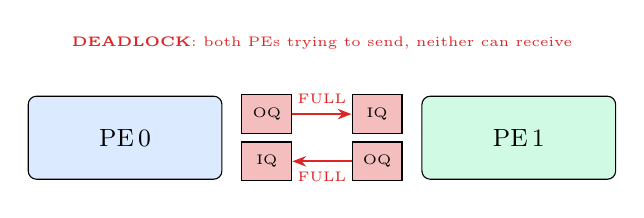
\begin{tikzpicture}[
    pe/.style={draw, rounded corners=3pt, minimum width=70pt, minimum height=30pt, font=\small},
    fifo/.style={draw, fill=#1, minimum width=18pt, minimum height=14pt, font=\tiny},
    arrow/.style={-{Stealth[length=5pt]}, thick},
  ]
  \node[pe, fill=pe0color] (pe0) at (0,0) {PE\,0};
  \node[pe, fill=pe1color] (pe1) at (5,0) {PE\,1};

  % Output FIFOs
  \node[fifo=conflictRed!30] (oq0) at (1.8,0.3) {OQ};
  \node[fifo=conflictRed!30] (oq1) at (3.2,0.3) {IQ};

  \node[fifo=conflictRed!30] (oq1b) at (3.2,-0.3) {OQ};
  \node[fifo=conflictRed!30] (iq0) at (1.8,-0.3) {IQ};

  % Arrows
  \draw[arrow, conflictRed] (oq0.east) -- (oq1.west) node[midway, above, font=\tiny] {FULL};
  \draw[arrow, conflictRed] (oq1b.west) -- (iq0.east) node[midway, below, font=\tiny] {FULL};

  % Labels
  \node[font=\tiny, conflictRed, anchor=south] at (2.5, 1) {\textbf{DEADLOCK}: both PEs trying to send, neither can receive};
\end{tikzpicture}
\end{center}

The deadlock scenario:
\begin{enumerate}[nosep]
  \item PE\,0 starts bulk DMA east $\to$ fills its output queue
  \item PE\,1 simultaneously starts bulk DMA west $\to$ fills its output queue
  \item PE\,0's output stalls because PE\,1's input queue is full (PE\,1 is busy sending, not draining receives)
  \item PE\,1's output stalls for the same reason (PE\,0 is busy sending, not draining receives)
  \item Neither PE can make progress $\Longrightarrow$ \textbf{deadlock}
\end{enumerate}

With \texttt{@mov32(.async = true)}, the DMA engine takes over the PE---once started, no other tasks (including receive handlers) can interleave until the DMA finishes or yields. When \emph{both} PEs in a pair fire bulk sends at the same time, neither can drain incoming wavelets, and the output FIFOs jam.

This problem gets \emph{worse} with graph density: our 12-node test has 30 boundary edges per PE. Trying to DMA 30 wavelets in one burst guarantees FIFO overflow when the neighbor is doing the same thing.

\subsection{Iteration 2: 2D Extension (Same Problem, Worse)}

The second version (\texttt{pe\_program.csl.pre-sync.bak}) added 2D grids with north/south support, but \textbf{kept the same bulk DMA approach}. With four directions instead of two, things got worse:

\begin{lstlisting}[language=CSL, numbers=none, caption={Pre-sync 2D version: still bulk DMA per direction}]
@mov32(east_out,  east_src,  .{ .async = true });
@mov32(west_out,  west_src,  .{ .async = true });
@mov32(south_out, south_src, .{ .async = true });   // NEW
@mov32(north_out, north_src, .{ .async = true });   // NEW
\end{lstlisting}

Four simultaneous async DMAs competing for fabric bandwidth, each potentially blocking on a different neighbor's full input queue. The deadlock window grew from two directions to four.

\subsection{Iteration 3: Sync Barrier (Addressed Timing, Not Backpressure)}

The third version (\texttt{pe\_program.csl.sync}) added the hardware row-reduce/broadcast barrier, correctly solving the \emph{synchronization} problem (making sure all PEs finish sending before detect/resolve runs). But it still used bulk DMA for the sends themselves. The barrier got the sequencing right, but could not prevent the FIFO deadlock during the send phase.

\subsection{V1--V3 Wavelet Format and Routing}

These early versions used a hop-count-based wavelet format with an 8-bit Manhattan hop field:

\begin{center}
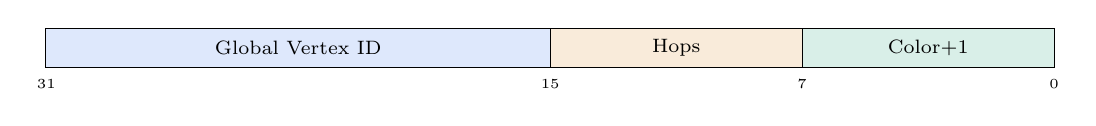
\begin{tikzpicture}[scale=0.4]
  \draw[thick] (0,0) rectangle (32,1.2);
  \fill[cpuBlue!15] (0,0) rectangle (16,1.2);
  \fill[warnOrange!15] (16,0) rectangle (24,1.2);
  \fill[confirmGreen!15] (24,0) rectangle (32,1.2);

  \draw (16,0)--(16,1.2);
  \draw (24,0)--(24,1.2);

  \node[font=\scriptsize] at (8, 0.6) {Global Vertex ID};
  \node[font=\scriptsize] at (20, 0.6) {Hops};
  \node[font=\scriptsize] at (28, 0.6) {Color+1};

  \node[font=\tiny, anchor=north] at (0, -0.1) {31};
  \node[font=\tiny, anchor=north] at (16, -0.1) {15};
  \node[font=\tiny, anchor=north] at (24, -0.1) {7};
  \node[font=\tiny, anchor=north] at (32, -0.1) {0};
\end{tikzpicture}
\end{center}

The boundary table included a fourth field, \texttt{boundary\_hops[b]}, encoding the Manhattan L-route. The host precomputed horizontal/vertical hop counts so relay PEs could decrement them in-flight:

\begin{lstlisting}[language=Python, caption={Hops computation (V1--V3)}, label=lst:hops]
def make_hops(h_dir, h_hops, v_dir, v_hops):
    return (h_dir << 7) | (h_hops << 4) | (v_dir << 3) | v_hops
\end{lstlisting}

\begin{lstlisting}[language=CSL, caption={Wavelet packing (V1--V3)}, label=lst:pack:old]
fn pack_wavelet(gid: i32, col: i32, hops: i32) u32 {
    const id_part   = @as(u32, @as(u16, gid));
    const hops_part = @as(u32, @as(u16, hops)) & 0xFF;
    const col_part  = @as(u32, @as(u16, col + 1)) & 0xFF;
    return (id_part << 16) | (hops_part << 8) | col_part;
}
\end{lstlisting}

The receive handler had to check for done sentinels, decrement hops, and handle corner turns for 2D routing---far more complex than the current stateless design:

\begin{lstlisting}[language=CSL, caption={East receive handler (V1--V3)}, label=lst:recv:old]
task recv_east(wval: u32) void {
    if (is_done_sentinel(wval)) {
        done_count += 1;
        if (unpack_h_hops(wval) > 0 and !is_west_edge)
            buffer_relay_west(dec_h_hops(wval));
    } else {
        const hh = unpack_h_hops(wval);
        if (hh > 0) {
            buffer_relay_west(dec_h_hops(wval));
        } else if (unpack_v_hops(wval) == 0) {
            process_incoming_wavelet(
                unpack_gid(wval), unpack_color(wval));
        } else {
            // Corner PE: turn from horizontal to vertical
        }
    }
    check_completion();
}
\end{lstlisting}

Done sentinels used a special GID = \texttt{0xFFFF} and were broadcast to all PEs ($O(P^2)$ sentinel traffic system-wide):

\begin{lstlisting}[language=CSL, numbers=none, caption={Done sentinel (V1--V3 broadcast-style)}]
fn make_done_wavelet(hops: i32) u32 {
    const hops_part = @as(u32, @as(u16, hops)) & 0xFF;
    return @as(u32, 0xFFFF0000) | (hops_part << 8);
}
\end{lstlisting}

This hop-count approach limited scalability to grid sizes where hop counts fit in 3~bits per axis, required host-side precomputation, and made the receive path complex. All of this was eliminated in V4's stateless GID-based routing.

\subsection{Iteration 4: The Cooperative Solution (Current)}
\label{sec:cooperative}

The current version solves the backpressure problem with three interlocking mechanisms:

\paragraph{(a) One-per-activation send chain.}
Instead of bulk DMA, we send \textbf{exactly one wavelet per task activation}. After each send, the task re-activates itself. Between activations, the PE's task scheduler can run pending receive tasks, draining input FIFOs:

\begin{lstlisting}[language=CSL, caption={Current approach: one wavelet per activation}, label=lst:onesend]
// Send state machine: wavelets are sent one-per-task-activation
// to avoid output FIFO deadlock. Between activations, recv data
// tasks can fire, draining input FIFOs and preventing circular
// backpressure.
task send_wavelet() void {
    if (drain_one_relay()) {       // priority: relay first
        @activate(send_wavelet_task_id);
        return;
    }
    if (send_phase == 0 and send_idx < east_count) {
        send_wavelet_east(east_send_buf[send_idx]);
        send_idx += 1;
        @activate(send_wavelet_task_id);   // re-arm
        return;
    }
    // ... next phase ...
}
\end{lstlisting}

The key insight: \texttt{@activate()} hands control back to the task scheduler. If a receive task is pending (a wavelet arrived on an input queue), it runs \emph{before} the next \texttt{send\_wavelet} activation. This interleaving guarantees input FIFOs get drained even while the PE is sending.

\paragraph{(b) Relay queues decouple receive from send.}
When a receive handler gets a wavelet that needs forwarding (multi-hop relay), it does \textbf{not} write to the output FIFO directly. Instead, it buffers the wavelet in a software relay queue:

\begin{lstlisting}[language=CSL, numbers=none]
// Relay queues: recv handlers buffer wavelets here for
// deferred forwarding. Decouples recv (input) from send
// (output), preventing circular deadlock.
// Implemented as circular ring buffers so drained slots are
// reused within a round.
var relay_east_q: [max_relay]u32;
var relay_east_head: u16 = 0;   // next drain position
var relay_east_tail: u16 = 0;   // next write position
var relay_east_count: u16 = 0;  // items currently buffered
\end{lstlisting}

Only the \texttt{send\_wavelet} task reads from relay queues and writes to output FIFOs. This prevents the scenario where a receive handler tries to write to a full output FIFO, which would block it and stop further input queue draining.

\paragraph{Circular ring buffers.}
An earlier version used \emph{linear} append-only relay buffers with separate read (\texttt{sent}) and write (\texttt{len}) pointers that only advanced forward. Once the \texttt{send\_wavelet} task drained a slot, that slot was wasted---new arrivals could only append past the end. If more relay wavelets arrived between drain opportunities than the buffer could hold, they were \textbf{silently dropped}.

The current implementation uses \emph{circular} ring buffers: drained slots wrap around and become available for new arrivals. A buffer of depth $N$ can now handle unlimited total relay throughput as long as no more than $N$ are in-flight at any instant:

\begin{lstlisting}[language=CSL, numbers=none]
fn buffer_relay_east(wval: u32) void {
    if (relay_east_count < max_relay) {
        relay_east_q[relay_east_tail] = wval;
        relay_east_tail += 1;
        if (relay_east_tail >= max_relay) relay_east_tail = 0;
        relay_east_count += 1;
    }
    @activate(send_wavelet_task_id);  // wake drain
}
fn drain_one_relay() bool {
    if (relay_east_count > 0) {
        send_wavelet_east(relay_east_q[relay_east_head]);
        relay_east_head += 1;
        if (relay_east_head >= max_relay) relay_east_head = 0;
        relay_east_count -= 1;
        return true;
    }
    // ... west, south, north ...
}
\end{lstlisting}

The buffer depth \texttt{max\_relay} is computed by the host at compile time. It analyzes every PE's relay load by tracing all boundary wavelets through their Manhattan routes and counting how many pass through each intermediate PE per direction. For example, with our 12-node graph on 4~PEs, the middle PEs (PE\,1 and PE\,2) each relay up to 20 wavelets per direction per round, so \texttt{max\_relay=20}. With only 2 PEs (adjacent, no relay needed), \texttt{max\_relay=1}.

\paragraph{Relay buffer overflow and the liveness problem.}
Even with circular ring buffers, the relay queue has a fixed depth. If wavelets arrive faster than they can be drained---or if a burst of relay traffic exceeds \texttt{max\_relay} slots---incoming wavelets are \textbf{silently dropped}. We track this with a per-PE overflow counter:

\begin{lstlisting}[language=CSL, numbers=none]
fn buffer_relay_east(wval: u32) void {
    if (relay_east_count < max_relay) {
        relay_east_q[relay_east_tail] = wval;
        relay_east_tail += 1;
        if (relay_east_tail >= max_relay) relay_east_tail = 0;
        relay_east_count += 1;
    } else {
        perf_counters[7] += 1;   // relay_overflow_drops
    }
    @activate(send_wavelet_task_id);
}
\end{lstlisting}

The host reads \texttt{perf\_counters[7]} after each run and reports any drops. But the real hazard is \textbf{liveness}: if a data wavelet is dropped, the destination PE waits forever for \texttt{data\_recv\_remaining} to reach zero---it never does, and the whole computation hangs.

\paragraph{(c) Completion detection: count-based with done sentinel fallback.}

The primary completion mechanism is \textbf{count-based}: the host precomputes \texttt{expected\_data\_recv} (the total number of data wavelets each PE should receive) and uploads it with the graph data. Each receive handler decrements \texttt{data\_recv\_remaining}; when it hits zero, data exchange is complete.

To guard against relay overflow, every PE also sends \textbf{done sentinels}---lightweight wavelets sent to each unique destination PE after all data wavelets have been transmitted. A done sentinel uses the same wavelet format but with $\texttt{color} = -1$ (which encodes as $-1+1=0$ in the 5-bit color field). The host precomputes \texttt{expected\_done\_recv} for each PE: the count of unique source PEs that send data to it.

\begin{lstlisting}[language=CSL, numbers=none, caption={Done sentinel construction (from \texttt{send\_boundary})}]
// Build dedup'd sentinel list: one per unique destination PE
var i: i16 = 0;
while (i < max_boundary) : (i += 1) {
    if (i >= nbnd) break;
    const gid = boundary_neighbor_gid[i];
    const dest = gid & pe_mask[0];
    if (dest != pe_id and done_sent_flags[dest] == 0) {
        done_send_buf[done_send_count] =
            pack_wavelet(pe_id, dest, -1);  // color = -1
        done_send_dir[done_send_count] =
            boundary_direction[i];          // initial direction
        done_send_count += 1;
        done_sent_flags[dest] = 1;
    }
}
\end{lstlisting}

The done sentinels are sent in \textbf{phase~4} of the send chain (after all data phases 0--3), so they always arrive \emph{after} the last data wavelet from that source PE. On the receive side, a sentinel increments \texttt{done\_recv\_count} rather than decrementing \texttt{data\_recv\_remaining}. The dual-path \texttt{check\_completion()} (shown earlier) uses both counters:

\begin{itemize}[nosep]
  \item \textbf{Normal path}: \texttt{data\_recv\_remaining $\leq$ 0} --- all data arrived.
  \item \textbf{Overflow recovery}: \texttt{done\_recv\_count $\geq$ expected\_done\_recv} --- all senders finished but some data was lost in relay buffers. The PE proceeds with whatever colors it did receive; the missing vertices will be re-colored in the next BSP round.
\end{itemize}

This guarantees the algorithm makes progress even when relay buffers overflow. In practice, overflow is rare: for our test suite of 9 graphs on 8 PEs, all runs report zero \texttt{relay\_overflow\_drops}. But the sentinel mechanism ensures we never hang if it does happen.

\subsection{Summary of Design Evolution}

\begin{center}
\renewcommand{\arraystretch}{1.3}
\begin{tabular}{p{42pt}p{85pt}p{70pt}p{70pt}p{80pt}}
\toprule
\textbf{Version} & \textbf{Send Strategy} & \textbf{Barrier} & \textbf{Multi-hop} & \textbf{Problem} \\
\midrule
V1 (1D) & Bulk \texttt{@mov32} async & Wavelet counting & No & FIFO deadlock \\
V2 (2D) & Bulk \texttt{@mov32} $\times$4 dirs & Wavelet counting & No & Worse deadlock \\
V3 (sync) & Bulk \texttt{@mov32} async & HW row-reduce + broadcast & No & Deadlock still possible \\
V4a & One-per-activation & HW barrier + done sentinels & Yes (relay queues) & Extra sentinel traffic \\
V4b & One-per-activation & HW barrier + count-based & Yes (relay queues) & Hangs on relay overflow \\
\textbf{V4c (current)} & \textbf{One-per-activation} & \textbf{HW barrier + count + sentinels} & \textbf{Yes (circular relay)} & \textbf{Deadlock-free + overflow-safe} \\
\bottomrule
\end{tabular}
\end{center}

The performance cost of one-per-activation sending is higher latency per wavelet (one task switch per wavelet instead of one DMA for the whole batch). But correctness is non-negotiable: a deadlocked program produces no result at all. In practice, the task-switch overhead is roughly 10--20 cycles per wavelet---negligible compared to fabric routing latency. And for large graphs with many boundary edges, the interleaved send/recv pattern actually gets \emph{better} sustained throughput than bulk DMA, because input FIFOs never fill up and fabric backpressure never kicks in.

%======================================================================
\section{Scaling to WSE-3: Limitations and Path Forward}
\label{sec:scaling}
%======================================================================

The current implementation runs correctly on small PE grids (up to $\sim$100~PEs)
and handles all test graphs without deadlock or data loss.
However, the WSE-3 fabric contains roughly 900{,}000 processing elements,
and several design choices that work fine at small scale
become fundamental bottlenecks at that size.
This section catalogs the limitations we have identified,
traces them to their root cause,
and outlines the changes needed to reach full-fabric scale.

\subsection{The Root Cause: Hash Partitioning Destroys Locality}

Before diving into individual issues, it helps to understand
why so many of them share a single root cause.

Our current partitioning strategy assigns vertex $v$ to PE
$v \mathbin{\&} (\mathit{total\_PEs}-1)$.
This is fast and simple, but it completely ignores the graph's structure:
two adjacent vertices can end up on opposite corners of the fabric.
On a 948$\times$948 grid, that means a single wavelet may travel
up to 1{,}896 relay hops---through nearly every PE on the grid---just
to reach its neighbor.

This one decision amplifies ten of the sixteen scaling problems we have cataloged.
Replacing hash partitioning with \textbf{locality-aware partitioning}
(e.g., METIS graph partitioning combined with Hilbert-curve spatial mapping)
is therefore the single highest-leverage change.
It reduces typical hop distance from $O(\mathit{grid\_dim})$ to $O(1\text{--}5)$,
shrinks boundary tables, limits the number of distinct destination PEs,
and eliminates the power-of-2 constraint on PE count.

\subsection{Priority~0 --- Will Not Compile at Scale}

\paragraph{(1) \texttt{done\_send\_buf} grows with total PEs.}
After sending data wavelets, each PE sends a ``done'' sentinel
to every unique destination PE.
The buffer that holds these sentinels (\texttt{done\_send\_buf})
is currently sized at \texttt{max\_boundary}---which, under hash partitioning,
can approach $P$ (the total PE count).
At 900K~PEs this alone would exceed the 48\,KB SRAM budget.
With locality-aware partitioning, the number of unique destination PEs
drops to a small constant (typically $<$50), making a fixed-size buffer feasible.

\paragraph{(2) \texttt{i16} types overflow at vertex counts above 32{,}767.}
Loop indices and array lengths throughout the PE kernel
(\texttt{pe\_program.csl}) are declared as \texttt{i16},
which silently overflows when the global vertex count exceeds 32{,}767.
The fix is mechanical: widen to \texttt{i32} everywhere.

\paragraph{(3) Wavelet encoding has only 11~bits for destination PE.}
The current encoding packs sender GID, destination PE,
and color into a single 32-bit wavelet as
$[\text{31:16}] = \text{sender\_gid}$, $[\text{15:5}] = \text{dest\_pe}$,
$[\text{4:0}] = \text{color}+1$.
Eleven bits address at most 2{,}048~PEs.
With locality-aware partitioning, the destination can be encoded as
a relative $(dx,\,dy)$ offset from the sender---6~bits each for modest hop distances---freeing
the remaining bits for a wider color field or sender ID.

\paragraph{(4) Layout generation uses a compile-time loop over all PEs.}
\texttt{layout.csl} instantiates each PE via a CSL \texttt{comptime} loop.
The compiler must unroll this loop entirely at compile time;
at 900K iterations, compilation time and memory become untenable.
CSL's \texttt{@set\_tile\_code} with a \texttt{.params} map
can replace the per-PE loop with a single parameterized tile,
letting the compiler generate one template and stamp it across the grid.

\subsection{Priority~1 --- Will Compile but Produce Wrong Results}

\paragraph{(5) No two-dimensional barrier.}
The current barrier uses east-to-west row-reduce followed by
west-to-east broadcast---a 1D scheme that only synchronizes within a single row.
In a 2D grid, PEs in different rows can drift out of phase,
leading to wavelet races between BSP rounds.
A proper 2D barrier requires adding a column-wise reduction
(south-to-north reduce, then north-to-south broadcast)
after the row-wise pass.

\paragraph{(6) Hash partitioning is the root cause of most scaling issues.}
As discussed above, replacing $\texttt{gid} \mathbin{\&} \texttt{pe\_mask}$
with METIS partitioning is the foundational change.
METIS minimizes edge cuts across partitions while balancing load,
and a Hilbert-curve or strip-map assignment places neighboring partitions
on physically adjacent PEs.

\paragraph{(7) Relay buffers can overflow under heavy pass-through traffic.}
Central PEs in the grid may have to relay wavelets from hundreds of crossing paths.
Even with circular ring buffers, a fixed depth of \texttt{max\_relay}
cannot absorb arbitrarily large bursts.
Locality-aware partitioning all but eliminates this problem
by keeping most wavelets within a small neighborhood.

\paragraph{(8) Uniform array sizing wastes SRAM on lightly loaded PEs.}
Every PE allocates arrays for \texttt{max\_local\_verts} vertices
regardless of how many it actually holds.
Under hash partitioning, the maximum can be 3--5$\times$ the average.
METIS balances partition sizes, bringing the max/avg ratio close to 1.0
and recovering significant SRAM headroom.

\subsection{Priority~2 --- Performance Bottlenecks}

\paragraph{(9) Linear search in \texttt{global\_to\_local}.}
Every adjacency lookup during speculation walks the \texttt{global\_vertex\_ids}
array linearly.
At 50 local vertices with average degree~20,
that is $\sim$50{,}000 scans per round per PE.
If METIS assigns contiguous GID ranges,
a direct index $\texttt{gid} - \texttt{min\_gid}$ gives $O(1)$ lookup.

\paragraph{(10) Incoming-wavelet processing scans the full boundary table.}
\texttt{process\_incoming\_wavelet} walks every boundary entry
for each arriving wavelet, at cost $O(B \times R)$ per round.
Sorting the boundary table by neighbor GID
and using binary search reduces this to $O(R \log B)$.

\paragraph{(11) Relay hops scale with grid dimension.}
Each software-relay hop involves a full task activation cycle.
On a 948$\times$948 grid, worst-case path length is 1{,}896 hops.
Locality-aware routing reduces this to typical 1--5~hops.

\paragraph{(12) Division via repeated subtraction for 2D routing.}
Converting a linear PE~ID to $(row, col)$ uses a loop
of $O(\mathit{num\_rows})$ subtractions.
If the column count is a power of 2,
a bit-shift gives the same result in $O(1)$.
With relative offsets from locality-aware encoding, the division is unnecessary entirely.

\subsection{Priority~3 --- Host-Side Preprocessing}

\paragraph{(13) Sequential per-PE H2D transfers.}
The host currently makes 12 blocking \texttt{memcpy\_h2d} calls per PE.
At 900K~PEs, that is 10.8~million sequential API calls.
Packing per-PE data into 3D tensors
$[\mathit{num\_rows}][\mathit{num\_cols}][\mathit{max\_size}]$
and issuing one rectangular transfer per symbol
reduces the call count to $\sim$12.

\paragraph{(14) Power-of-2 PE count constraint.}
Hash partitioning requires $\texttt{total\_PEs}$ to be a power of two.
The WSE-3 has $\sim$900K~PEs,
so the nearest valid count (524{,}288) wastes 42\% of the fabric.
METIS partitioning imposes no such constraint.

\paragraph{(15) $O(n^2)$ conflict-graph construction.}
The host builds the Pauli conflict graph by checking every pair of strings.
For large inputs, this dominates preprocessing time.
Vectorized numpy or the existing \texttt{graph\_builder.py} CSR path are faster alternatives.

\paragraph{(16) JSON serialization at scale.}
Graph partition data for 900K~PEs, serialized as JSON,
can reach gigabytes.
Switching to numpy \texttt{.npz} or HDF5 format
offers 10--100$\times$ speed-up and far smaller files.

\subsection{SRAM Budget After Locality-Aware Fixes}

With METIS partitioning, $\sim$10-hop max relay distance,
and $\sim$20 boundary edges on average, the per-PE memory budget fits comfortably:

\begin{center}
\renewcommand{\arraystretch}{1.2}
\begin{tabular}{lrl}
\toprule
\textbf{Array} & \textbf{Bytes} & \textbf{Notes} \\
\midrule
\texttt{csr\_offsets} & 204 & $51 \times 4$ \\
\texttt{csr\_adj} & 2{,}000 & $500 \times 4$ \\
\texttt{colors} + \texttt{tentative} & 400 & $50 \times 4 \times 2$ \\
\texttt{global\_vertex\_ids} & 200 & $50 \times 4$ \\
\texttt{boundary\_*} (3 arrays) & 600 & $50 \times 4 \times 3$ \\
\texttt{remote\_recv\_color} & 200 & $50 \times 4$ \\
\texttt{*\_send\_buf} (4 dirs) & 800 & $50 \times 4 \times 4$ \\
\texttt{relay\_*\_q} (4 dirs) & 1{,}024 & $64 \times 4 \times 4$ \\
Done tracking (fixed-size set) & 384 & $64 \times 6$ \\
\texttt{forbidden} & 128 & $32 \times 4$ \\
GID$\to$local hash table & 1{,}024 & $128 \times 8$ \\
Misc (perf, timer, etc.) & 200 & \\
\midrule
\textbf{Total} & \textbf{$\sim$7.2\,KB} & \\
\bottomrule
\end{tabular}
\end{center}

This leaves roughly 40.8\,KB of headroom out of the 48\,KB per-PE SRAM---ample
room for larger local subgraphs or additional bookkeeping.

\subsection{Recommended Implementation Order}

The dependencies between these fixes suggest a natural sequence:

\begin{enumerate}[nosep]
  \item \textbf{Locality-aware partitioning} (\#6): foundational change that reduces the severity of ten other issues.
  \item \textbf{Widen types to \texttt{i32}} (\#2): mechanical, required for compilation at scale.
  \item \textbf{Fix layout compile-time loop} (\#4): also required for compilation at scale.
  \item \textbf{Redesign wavelet encoding} (\#3): leverage locality for compact relative offsets.
  \item \textbf{Replace \texttt{done\_send\_buf}} (\#1): now feasible because locality limits the destination set.
  \item \textbf{Bulk H2D transfers} (\#13): independent host-side change, can proceed in parallel.
  \item \textbf{Implement 2D barrier} (\#5): correctness fix for full 2D mode.
  \item \textbf{Optimize lookups} (\#9, \#10): performance polish, lowest priority.
\end{enumerate}

\end{document}
